\documentclass{article}
\usepackage{neurips_2026}
\usepackage[utf8]{inputenc}
\usepackage[T1]{fontenc}
\usepackage{hyperref}
\usepackage{url}
\usepackage{booktabs}
\usepackage{amsfonts,amsmath,amssymb,amsthm}
\usepackage{nicefrac}
\usepackage{microtype}
\usepackage{xcolor}
\usepackage{graphicx}

\newtheorem{proposition}{Proposition}
\newtheorem{remark}{Remark}
\newcommand{\E}{\mathbb{E}}
\newcommand{\tr}{\operatorname{tr}}
\newcommand{\rmse}{\mathrm{RMSE}_z}

\title{How many benchmarks must be run? Selecting benchmarks and inferring the rest of a model's scores from a public score matrix}

\author{Anonymous Author(s)}

\begin{document}
\maketitle

\begin{abstract}
Evaluating a model on every benchmark of a large suite is costly, yet public leaderboards hold many ``model $\times$ benchmark'' score records. We ask: if only $k$ benchmarks can be run for a new model, which $k$ should they be, how should the remaining scores be inferred, and how large must $k$ be? We study this on real, partially observed score matrices (MTEB embedding results at three data densities, Open LLM Leaderboard v2, HELM Lite, LiveBench) with a held-out-\emph{model} protocol in which whole model families are held out and the choice of the $k$ benchmarks never sees the held-out scores. We compare random subsets with greedy designs derived from a latent-factor model (Bayesian I-optimal design) and from an empirical Gaussian covariance (greedy variance reduction), and with k-means, pivoted-QR and communality-ranked choices, using factor-analysis, Gaussian-conditional and kNN predictors, and report family-cluster-bootstrap intervals. We also derive the error of random-subset prediction under a Gaussian factor model: an exact finite-$k$ formula for least squares, a Jensen lower bound and a Marchenko--Pastur deterministic equivalent (1.4\% median error against simulation) for the Bayes predictor, and we check it on real matrices. Findings: (i) the matrices are strongly low-rank-dominated (first PC 56--73\% of variance) and, on MTEB, a random subset of 3--4 benchmarks closes half of the gap between the no-information baseline and the error reached with $k=24$--$48$, while 8--16 are needed for 80\%; (ii) choosing benchmarks matters most at small $k$ (6--20\% lower median error than random at $k\le4$) but the advantage of factor-model designs fades beyond $k\approx8$--$16$, where the covariance-based greedy rule keeps a 6--19\% edge and communality ranking becomes \emph{worse} than random (+4 to +13\%); (iii) the theory predicts the measured random-subset error curve of the factor predictor on MTEB to within about 20--35\% but is pessimistic (measured 23--32\% below implied) at $k=1$ on the small LLM leaderboards; (iv) the benefit of designed subsets survives training on only $\approx$15 models but the pairwise-covariance predictor collapses when 80\% of training cells are missing, while the EM factor model degrades gracefully. The LLM-leaderboard matrices have only 6--10 benchmarks, so our conclusions about $k$ for generative LLMs are limited to $k\le6$.
\end{abstract}

\section{Introduction}
Public leaderboards accumulate a ``model $\times$ benchmark'' score matrix in which scores of different benchmarks are far from independent. An evaluator who must assess a new model but can afford to run only $k$ of the $N$ benchmarks faces three linked questions: \emph{which} $k$ benchmarks to run, \emph{how} to infer the other $N-k$ scores from them and from the historical matrix, and \emph{how large} $k$ has to be. Item-level subsampling within one benchmark has been studied \citep{polo2024tiny,vivek2024anchor,kipnis2024metabench}; here we study the complementary benchmark-level problem, with the unit of selection being an entire benchmark (or task), and the unit of evaluation being a held-out \emph{model}.

We state three hypotheses before running experiments. \textbf{H1} (low effective rank): because score matrices are dominated by a few latent factors, a small $k$ suffices for most of the attainable accuracy. \textbf{H2} (design matters): subsets chosen by an experimental-design criterion beat random subsets, with an advantage that is largest when $k$ is comparable to the effective rank and shrinks as $k$ grows. \textbf{H3} (theory): under a Gaussian factor model the error of random-subset prediction follows a closed-form curve with a transition near $k\approx r$, and this curve describes real matrices. \textbf{H4} (data conditions): the conclusions hold when the history is small or sparse, but only for predictors that handle missing data properly.

\paragraph{Contributions.} (1) A held-out-model, held-out-family evaluation protocol for benchmark-subset selection in which selection is blind to the new model's scores and hyper-parameters are tuned on training rows only. (2) A comparison of six selection rules and six predictors on six real matrices with cluster-bootstrap uncertainty. (3) Derivations of the random-subset error (Section~\ref{sec:theory}) with synthetic verification and a check against real matrices, including where it fails. (4) A candid account of where the conclusions do and do not hold: they are supported on embedding benchmarks with up to 357 benchmarks, and only weakly testable on generative-LLM leaderboards that have 6--10 benchmarks.

\section{Related work}
\textbf{Few-example evaluation.} tinyBenchmarks selects or reweights evaluation \emph{items} to estimate a model's accuracy on one benchmark \citep{polo2024tiny}; Anchor Points clusters items by model-confidence patterns \citep{vivek2024anchor}; metabench distills six benchmarks into a sparse benchmark from the evaluations of thousands of models \citep{kipnis2024metabench}. Our unit of selection is a whole benchmark and the target is the model's score on the \emph{other} benchmarks.
\textbf{Cross-benchmark structure.} BenchBench studies whether benchmarks agree and how methodological choices change that conclusion \citep{perlitz2024benchbench}; observational scaling laws explain scores on many benchmarks through a low-dimensional capability space estimated from public models \citep{ruan2024observational}; Sloth fits skill-based scaling laws to predict multi-benchmark performance across families \citep{polo2024sloth}. These works show that benchmark scores share a low-dimensional structure; we use the same structural assumption but ask the \emph{design} question (which benchmarks to run) and quantify error as a function of $k$.
\textbf{Statistical tools.} Factor analysis with missing data fit by EM \citep{rubin1982em,tipping1999ppca}, low-rank completion \citep{candes2012exact}, Bayesian optimal design \citep{chaloner1995bayesian} and greedy sensor placement in Gaussian models \citep{guestrin2005near} are the building blocks; the contribution here is their combination and empirical assessment in the benchmark-selection setting, not a new estimator. The benchmark suites we use are MTEB \citep{muennighoff2022mteb}, HELM \citep{liang2022helm}, the Open LLM Leaderboard and LiveBench.

\section{Problem, methods and theory}
\paragraph{Setting.} A historical matrix $Y\in\mathbb{R}^{M\times N}$ (NaN = missing) of $M$ models and $N$ benchmarks. A new model has an unknown score vector $y\in\mathbb{R}^N$, of which the benchmarks $C$ (those it has been evaluated on, in the data) are \emph{candidates}. The evaluator chooses $S\subset C$, $|S|=k$ using only $Y$ (selection is blind to $y$), observes $y_S$, and predicts $\hat y_T$ for $T=C\setminus S$. Columns are standardised with training-row statistics to $z$; error is $\rmse=\sqrt{\frac1{|T|}\sum_{j\in T}(\hat z_j-z_j)^2}$ per held-out model, i.e.\ in units of the across-model standard deviation of each benchmark (also reported in score points).

\paragraph{Predictors.} (a) \emph{Train mean} ($\hat z=0$; uses no scores; reference for ``no information''). (b) \emph{FA($r$)}: a factor model $z=Vu+\varepsilon$, $u\sim\mathcal N(0,I_r)$, $\varepsilon_j\sim\mathcal N(0,\psi_j)$, fit by EM on the incomplete training matrix (80 EM iterations, SVD initialisation, loadings ridge $10^{-2}$, $\psi_j\ge0.02$; $r\in\{1,2,3,4,6,8,12,16,24\}$, $\alpha\in\{.02,.05,.1,.2,.4\}$), prediction $=V\,\E[u\mid z_S]$. (c) \emph{Gauss-cov}: the Gaussian conditional mean $\Sigma_{\cdot S}(\Sigma_{SS}+10^{-2}I)^{-1}z_S$ with $\Sigma$ a pairwise-complete correlation matrix (min.\ 15 shared models, projected to the PSD cone) shrunk towards identity by $\alpha$. (d) \emph{kNN}: mean of the $K{=}10$ training models closest on $S$. (e) PPCA (isotropic $\psi$) and a 1-factor model. $r$ and $\alpha$ are chosen per fold on a validation split of the training rows (random subsets of sizes spanning the $k$ grid).

\paragraph{Selection rules.} \emph{Random} (10 draws per model and $k$, averaged). \emph{Greedy I-opt}: with fitted $(V,\psi)$, the posterior covariance of $u$ is $\Sigma_S=(I+V_S^\top\Psi_S^{-1}V_S)^{-1}$; greedily add the benchmark minimising $\tr(V^\top V\,\Sigma_S)$, the total posterior variance of the signal over all benchmarks (Bayesian A-optimal design; rank-one updates; $O(Nkr^2)$). Nested in $k$. We claim no approximation guarantee. \emph{Greedy cov}: model-free greedy variance reduction on the shrunk correlation matrix, targets $=C$. \emph{Top communality}: rank benchmarks by $\|v_j\|^2/(\|v_j\|^2+\psi_j)$. \emph{Pivoted QR} on $\Psi^{-1/2}V$ (deterministic leverage-type selection; falls back to communality for $k>r$). \emph{k-means cover}: $k$ clusters in loading space, one member each. Each rule is restricted to the benchmarks the model was actually evaluated on.

\subsection{Theory: error of random subsets under a Gaussian factor model}\label{sec:theory}
Assume $z_j=v_j^\top u+e_j$, $u\sim\mathcal N(0,I_r)$, $e_j\sim\mathcal N(0,\sigma^2)$, loadings $v_j\overset{iid}{\sim}\mathcal N(0,I_r)$ known, and $S$ a uniformly random $k$-subset. Let $W=V_S^\top V_S\sim\mathrm{Wishart}_r(k,I)$.
\begin{proposition}[Exact error of least squares]\label{prop:ols}
With $\hat u=(V_S^\top V_S)^{-1}V_S^\top z_S$ and $k>r+1$, the expected squared error on a fresh benchmark is $\sigma^2\bigl(1+\tfrac{r}{k-r-1}\bigr)$; for $k\le r+1$ it is infinite (and for $k\le r$ the estimator is not defined).
\end{proposition}
\begin{proposition}[Bayes predictor]\label{prop:bayes}
With $\hat u=(\sigma^2I+W)^{-1}V_S^\top z_S$ the expected error is $\sigma^2+\E\,\tr\bigl[(I+W/\sigma^2)^{-1}\bigr]$, which (i) is at least $\sigma^2\bigl(1+\tfrac{r}{k+\sigma^2}\bigr)$ by Jensen (matrix inversion is operator convex), (ii) is finite for every $k\ge0$, (iii) satisfies, for $r,k\to\infty$ with $r/k\to c$, $\E\,\tr[(I+W/\sigma^2)^{-1}]\simeq r\lambda\,m(-\lambda)$ with $\lambda=\sigma^2/k$ and $m(-\lambda)=\frac{-(\lambda+1-c)+\sqrt{(\lambda+1-c)^2+4c\lambda}}{2c\lambda}$ the Stieltjes transform of the Marchenko--Pastur law \citep{marchenko1967distribution} at $-\lambda$. Limits: $\to\sigma^2r/k$ for $k\gg r$, and $\to r-k$ for $k\ll r$ with $\sigma^2\to0$.
\end{proposition}
Proofs are in Appendix~\ref{app:proofs}. The consequence for the evaluator is a \emph{phase transition} at $k\approx r$: below it, unresolved latent directions keep (nearly) their prior variance, above it the excess shrinks like $\sigma^2r/k$. For a \emph{given} subset, the error under a fitted factor model is $\frac1{|T|}\sum_{j\in T}\bigl(\psi_j+v_j^\top\Sigma_S v_j\bigr)$ (``model-implied error''), which is exactly the quantity that the I-opt rule minimises (up to the choice of $T$). When loadings are estimated from $M$ rows the error has an additional term, which we measure rather than derive (Appendix~\ref{app:synth}).

\section{Experimental protocol}\label{sec:protocol}
\paragraph{Data.} All from the pinned versions in \texttt{data.md}. \textbf{MTEB} (embeddings-benchmark/results at commit \texttt{6dabbcc}): one score per (model, task) = mean over subsets of \texttt{main\_score} on the test (else validation/dev) split, averaged over a model's result directories; tasks with $\ge100$ models and models with $\ge20$ such tasks give \emph{MTEB-wide} ($291\times357$, 58\% observed; the 234 models with $\ge45$ observed tasks are held out in turn, 70\% observed). Two complete sub-matrices are extracted from it by greedily deleting the row or column with most missing cells (row scores multiplied by $\alpha=1$ for \emph{MTEB-dense} and $\alpha=0.6$ for \emph{MTEB-mid}; see \texttt{data\_prep.py}): \emph{MTEB-dense} ($117\times287$) and \emph{MTEB-mid} ($139\times65$). \textbf{Open LLM Leaderboard v2} (4496 unflagged, de-duplicated models $\times$ 6 raw scores), \textbf{HELM Lite v1.13.0} ($91\times10$), \textbf{LiveBench} judgments (mean per model and task; 7 tasks, 195 models, 318 missing cells; models with $\ge6$ tasks evaluated). The three MTEB matrices are nested views of the same data, not independent replications; the LLM boards are independent but tiny in $N$.
\paragraph{Splits.} 10-fold cross-validation over \emph{models}. \emph{Family split} (primary): all models sharing a family key (organisation prefix for MTEB/OLB, first token of the model name for HELM/LiveBench) are held out together, folds balanced by size; \emph{random split} for comparison. For every held-out model and every $k$ in $\{1,2,3,4,5,6,8,10,12,16,20,24,\dots\}$ up to $k_{\max}$ (24, 48, 32, 3, 6, 4 for the six matrices) all rules choose $S$ from the model's observed benchmarks; the remaining observed ones are targets (at least 8 for MTEB, 3 for OLB/HELM, 2 for LiveBench; a held-out model must have observed at least $k_{\max}$ plus that many benchmarks, which is why MTEB-wide is restricted to models with $\ge45$ tasks). Standardisation, EM, correlation estimation, and the selection of $r,\alpha$ use training rows only.
\paragraph{Statistics.} Headline: median over held-out models of $\rmse$ (a few new-family models are gross outliers, so means are also reported in the repository and quoted where they differ), with 95\% percentile intervals from a cluster bootstrap over families (1000 resamples); paired comparisons use the same resamples. Wilcoxon signed-rank tests with Holm correction over all (matrix, split, rule, $k$) comparisons are descriptive only because models within a family are dependent. Fold-assignment seeds 0--2 are compared for MTEB-mid in Table~\ref{tab:seeds}. $k_{50}$/$k_{80}$ denote the smallest $k$ closing 50\%/80\% of the gap between the train-mean baseline and the error at $k_{\max}$ (so they depend on $k_{\max}$).

\section{Results}
\subsection{A few benchmarks carry most of the signal (H1)}
Table~\ref{tab:data} shows strong dominance of the first principal component (56--73\% of variance) and small participation ratios (1.8--3.0), although 90\% of variance needs 9--23 components on MTEB. Figure~\ref{fig:main} and Table~\ref{tab:mteb} show that the median $\rmse$ falls from 0.76--0.86 for the train-mean baseline to 0.43--0.55 at $k=8$ and 0.35--0.49 at $k=24$ on MTEB (family split; range over the three matrices and over random/designed subsets). Table~\ref{tab:kneeded}: random subsets need $k_{50}=3$--4 and $k_{80}=8$--16 on MTEB; in raw units (Table~\ref{tab:raw}) the median mean-absolute error on MTEB-mid drops from 9.6 score points (train mean) to 5.0 at $k=8$ with random choice and to 4.2--4.4 with a designed subset. On OLB/HELM/LiveBench, $k_{\max}=3,6,4$ already removes about 40\% (random subsets) to 55\% (greedy cov) of the baseline error (Table~\ref{tab:llm}), but $k_{\max}$ is so small that $k_{50}$ and $k_{80}$ there are weakly informative.
\begin{figure}[t]
\centering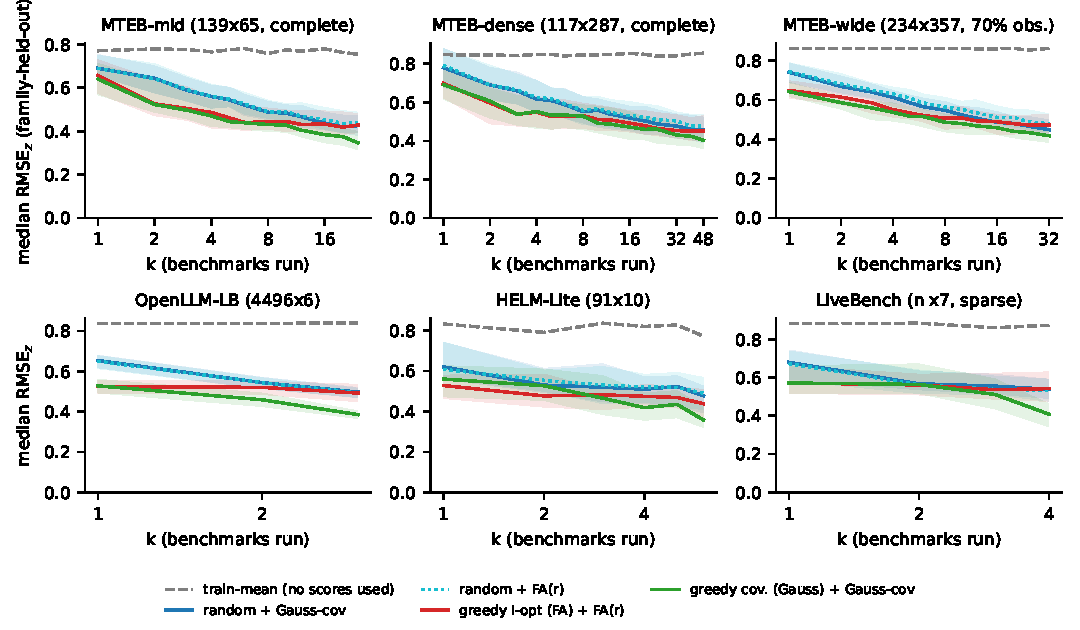
\includegraphics[width=\linewidth]{figs/fig_main_curves.pdf}
\caption{Median $\rmse$ over held-out models (family split) vs.\ number of benchmarks run $k$; bands: 95\% cluster-bootstrap CI. ``Train mean'' uses none of the new model's scores.}\label{fig:main}
\end{figure}
\begin{table}[t]
\caption{Matrix summaries (z-scored correlation spectrum; pairwise-complete correlations where cells are missing). MTEB-wide: 291 models, of which the 234 with $\ge45$ observed tasks serve as held-out models. $r_{80},r_{90}$: components for 80\%/90\% of variance.}\label{tab:data}
\centering\small\begin{tabular}{lrrrrrrr}\toprule
matrix & models & benchm. & observed & PC1 & $r_{80}$ & $r_{90}$ & part.\ ratio \\\midrule
MTEB-mid & 139 & 65 & 100\% & 0.62 & 4 & 9 & 2.5 \\
MTEB-dense & 117 & 287 & 100\% & 0.56 & 5 & 15 & 2.9 \\
MTEB-wide & 291 & 357 & 58\% & 0.56 & 8 & 23 & 3.0 \\
OpenLLM-LB & 4496 & 6 & 100\% & 0.73 & 2 & 3 & 1.8 \\
HELM-Lite & 91 & 10 & 100\% & 0.63 & 2 & 4 & 2.3 \\
LiveBench & 195 & 7 & 77\% & 0.73 & 2 & 4 & 1.8 \\
\bottomrule\end{tabular}

\end{table}
\begin{table}[t]
\caption{MTEB, family split: median $\rmse$ [95\% family-cluster CI] over held-out models.}\label{tab:mteb}
\centering\scriptsize\setlength{\tabcolsep}{3pt}\begin{tabular}{lrrrrrr}\toprule
$k$ & 1 & 2 & 4 & 8 & 16 & 24 \\\midrule
\multicolumn{7}{l}{\textit{MTEB-mid (139x65, complete)}} \\
train mean & 0.771 \scriptsize[0.657,0.960] & 0.779 \scriptsize[0.653,0.958] & 0.766 \scriptsize[0.657,0.951] & 0.759 \scriptsize[0.658,0.952] & 0.779 \scriptsize[0.655,0.959] & 0.754 \scriptsize[0.655,0.953] \\
random + Gauss & 0.690 \scriptsize[0.654,0.754] & 0.644 \scriptsize[0.577,0.701] & 0.560 \scriptsize[0.506,0.612] & 0.487 \scriptsize[0.453,0.538] & 0.437 \scriptsize[0.406,0.487] & 0.425 \scriptsize[0.381,0.470] \\
random + FA & 0.690 \scriptsize[0.656,0.750] & 0.641 \scriptsize[0.576,0.711] & 0.561 \scriptsize[0.506,0.616] & 0.489 \scriptsize[0.459,0.542] & 0.454 \scriptsize[0.409,0.510] & 0.441 \scriptsize[0.392,0.488] \\
greedy I-opt + FA & 0.656 \scriptsize[0.574,0.728] & 0.526 \scriptsize[0.471,0.641] & 0.486 \scriptsize[0.415,0.554] & 0.442 \scriptsize[0.409,0.507] & 0.433 \scriptsize[0.388,0.493] & 0.428 \scriptsize[0.394,0.481] \\
greedy cov + Gauss & 0.640 \scriptsize[0.568,0.713] & 0.523 \scriptsize[0.487,0.631] & 0.470 \scriptsize[0.422,0.544] & 0.431 \scriptsize[0.398,0.484] & 0.384 \scriptsize[0.347,0.439] & 0.347 \scriptsize[0.315,0.399] \\
\multicolumn{7}{l}{\textit{MTEB-dense (117x287, complete)}} \\
train mean & 0.847 \scriptsize[0.696,1.024] & 0.846 \scriptsize[0.697,1.021] & 0.849 \scriptsize[0.695,1.026] & 0.847 \scriptsize[0.697,1.025] & 0.854 \scriptsize[0.697,1.023] & 0.840 \scriptsize[0.694,1.027] \\
random + Gauss & 0.780 \scriptsize[0.679,0.879] & 0.690 \scriptsize[0.613,0.781] & 0.617 \scriptsize[0.550,0.713] & 0.552 \scriptsize[0.493,0.629] & 0.519 \scriptsize[0.452,0.580] & 0.489 \scriptsize[0.433,0.561] \\
random + FA & 0.791 \scriptsize[0.679,0.878] & 0.690 \scriptsize[0.615,0.792] & 0.626 \scriptsize[0.547,0.713] & 0.558 \scriptsize[0.483,0.630] & 0.530 \scriptsize[0.458,0.604] & 0.510 \scriptsize[0.451,0.583] \\
greedy I-opt + FA & 0.697 \scriptsize[0.624,0.773] & 0.597 \scriptsize[0.488,0.703] & 0.548 \scriptsize[0.472,0.627] & 0.530 \scriptsize[0.464,0.595] & 0.492 \scriptsize[0.446,0.556] & 0.464 \scriptsize[0.427,0.547] \\
greedy cov + Gauss & 0.691 \scriptsize[0.616,0.783] & 0.607 \scriptsize[0.518,0.674] & 0.552 \scriptsize[0.465,0.620] & 0.528 \scriptsize[0.458,0.586] & 0.471 \scriptsize[0.407,0.552] & 0.461 \scriptsize[0.388,0.514] \\
\multicolumn{7}{l}{\textit{MTEB-wide (234x357, 70\% obs.)}} \\
train mean & 0.861 \scriptsize[0.786,0.993] & 0.860 \scriptsize[0.785,0.993] & 0.861 \scriptsize[0.784,0.994] & 0.861 \scriptsize[0.784,0.988] & 0.860 \scriptsize[0.786,0.993] & 0.853 \scriptsize[0.780,0.991] \\
random + Gauss & 0.741 \scriptsize[0.688,0.787] & 0.669 \scriptsize[0.630,0.722] & 0.613 \scriptsize[0.567,0.647] & 0.547 \scriptsize[0.512,0.591] & 0.486 \scriptsize[0.457,0.540] & 0.468 \scriptsize[0.433,0.516] \\
random + FA & 0.743 \scriptsize[0.692,0.789] & 0.681 \scriptsize[0.636,0.734] & 0.630 \scriptsize[0.585,0.665] & 0.564 \scriptsize[0.527,0.613] & 0.512 \scriptsize[0.480,0.569] & 0.490 \scriptsize[0.450,0.550] \\
greedy I-opt + FA & 0.648 \scriptsize[0.609,0.698] & 0.614 \scriptsize[0.578,0.661] & 0.551 \scriptsize[0.513,0.614] & 0.507 \scriptsize[0.451,0.562] & 0.489 \scriptsize[0.426,0.526] & 0.473 \scriptsize[0.431,0.523] \\
greedy cov + Gauss & 0.642 \scriptsize[0.618,0.689] & 0.586 \scriptsize[0.553,0.620] & 0.537 \scriptsize[0.492,0.584] & 0.486 \scriptsize[0.438,0.528] & 0.458 \scriptsize[0.424,0.501] & 0.435 \scriptsize[0.397,0.477] \\
\bottomrule\end{tabular}

\end{table}

\subsection{Selection matters most at small $k$ (H2)}
Table~\ref{tab:selgain} and Figure~\ref{fig:gain} give the paired change of median error relative to random subsets under the same Gauss-cov predictor. On the three MTEB matrices both greedy rules beat random, with intervals excluding zero in 41 of 42 (matrix, rule, $k\le8$) cases (the exception is I-opt at $k=1$ on MTEB-mid, $[-17,+0.5]\%$); the median gain is 6--20\% at $k\le4$ and 4--12\% at $k=8$. Beyond $k\approx8$--$16$ the I-opt design, which is tailored to the rank-$r$ factor posterior, loses most of its edge (MTEB-mid: $-20\%$ at $k=2$ but $-3\%$ and $-5\%$ at $k=16,24$), whereas the model-free covariance greedy rule keeps $-6$ to $-19\%$. Pure communality ranking is the worst rule: it is better than random only at small $k$ on MTEB-mid (and not reliably elsewhere), and its point estimate is 4--13\% \emph{worse} than random at $k=16$ and 10--12\% worse at $k=24$ on the three MTEB matrices; inspection (Appendix~\ref{app:selected}) shows it picks near-duplicate tasks (six CQADupstack subforums on MTEB-dense), i.e.\ redundancy is the failure mode. Holm-corrected Wilcoxon tests find the greedy-cov advantage significant at all tested $k$ on the three MTEB matrices and the I-opt advantage at 36 of 40 $(\text{matrix},k)$ settings there (descriptive; Appendix~\ref{app:tests}). On the LLM boards, designed subsets at $k=1$ reduce error by 10--19\% (e.g.\ OLB: MMLU-PRO is picked first by both greedy rules), but intervals are wide for HELM and LiveBench and the advantage at larger $k$ is mixed (LiveBench $k=4$: pivoted QR $+13\%$, I-opt $-2\%$).
\begin{figure}[t]
\centering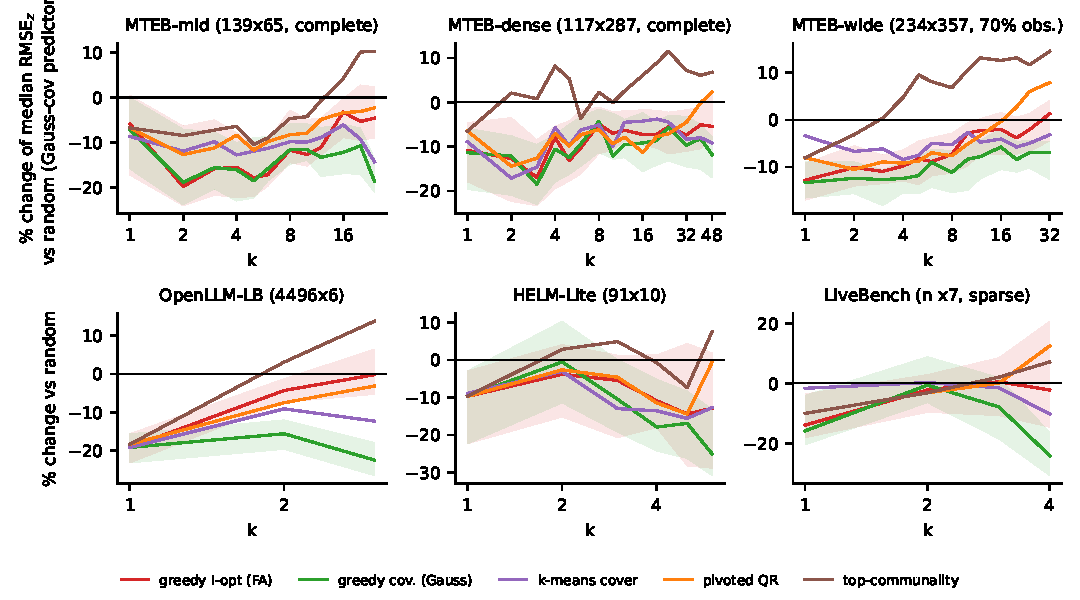
\includegraphics[width=\linewidth]{figs/fig_selection_gain.pdf}
\caption{Change (\%) of median $\rmse$ relative to random subsets (same Gauss-cov predictor), family split; bands: 95\% cluster-bootstrap CI for the two greedy rules.}\label{fig:gain}
\end{figure}
\begin{table}[t]
\caption{Selection rules vs.\ random (Gauss-cov predictor), family split: change of median $\rmse$ [95\% CI], percent.}\label{tab:selgain}
\centering\scriptsize\setlength{\tabcolsep}{2.5pt}\begin{tabular}{llrrrrr}\toprule
matrix & selection & $k$=2 & 4 & 8 & 16 & 24 \\\midrule
MTEB-mid & greedy cov & -19\% \scriptsize[-24,-7] & -16\% \scriptsize[-23,-10] & -12\% \scriptsize[-15,-6] & -12\% \scriptsize[-17,-6] & -19\% \scriptsize[-21,-13] \\
MTEB-mid & greedy I-opt & -20\% \scriptsize[-24,-6] & -15\% \scriptsize[-22,-8] & -12\% \scriptsize[-14,-3] & -3\% \scriptsize[-9,-0] & -5\% \scriptsize[-9,+2] \\
MTEB-mid & k-means cover & -12\% \scriptsize[-17,-5] & -13\% \scriptsize[-17,-6] & -10\% \scriptsize[-13,-5] & -6\% \scriptsize[-12,-3] & -14\% \scriptsize[-20,-8] \\
MTEB-mid & pivoted QR & -13\% \scriptsize[-17,-5] & -8\% \scriptsize[-17,-2] & -8\% \scriptsize[-11,-1] & -3\% \scriptsize[-8,+0] & -2\% \scriptsize[-8,+5] \\
MTEB-mid & top communality & -8\% \scriptsize[-15,-3] & -6\% \scriptsize[-14,-2] & -5\% \scriptsize[-8,+1] & +4\% \scriptsize[-1,+8] & +10\% \scriptsize[+5,+15] \\
MTEB-dense & greedy cov & -12\% \scriptsize[-21,-8] & -11\% \scriptsize[-18,-7] & -4\% \scriptsize[-11,-2] & -9\% \scriptsize[-16,-2] & -6\% \scriptsize[-13,-3] \\
MTEB-dense & greedy I-opt & -13\% \scriptsize[-22,-3] & -8\% \scriptsize[-19,-5] & -5\% \scriptsize[-12,-1] & -7\% \scriptsize[-10,-2] & -6\% \scriptsize[-12,-2] \\
MTEB-dense & k-means cover & -17\% \scriptsize[-25,-13] & -6\% \scriptsize[-14,-0] & -5\% \scriptsize[-11,-1] & -4\% \scriptsize[-7,+1] & -4\% \scriptsize[-9,-1] \\
MTEB-dense & pivoted QR & -14\% \scriptsize[-23,-8] & -7\% \scriptsize[-15,-5] & -6\% \scriptsize[-12,-3] & -11\% \scriptsize[-14,-4] & -7\% \scriptsize[-11,-1] \\
MTEB-dense & top communality & +2\% \scriptsize[-12,+15] & +8\% \scriptsize[-6,+24] & +2\% \scriptsize[-7,+6] & +6\% \scriptsize[-1,+10] & +11\% \scriptsize[+4,+18] \\
MTEB-wide & greedy cov & -12\% \scriptsize[-16,-9] & -12\% \scriptsize[-16,-9] & -11\% \scriptsize[-15,-7] & -6\% \scriptsize[-11,-2] & -7\% \scriptsize[-10,-4] \\
MTEB-wide & greedy I-opt & -10\% \scriptsize[-14,-5] & -10\% \scriptsize[-13,-6] & -7\% \scriptsize[-11,-3] & -2\% \scriptsize[-7,+2] & -2\% \scriptsize[-7,+1] \\
MTEB-wide & k-means cover & -7\% \scriptsize[-11,-3] & -8\% \scriptsize[-11,-3] & -5\% \scriptsize[-8,-1] & -4\% \scriptsize[-9,-2] & -5\% \scriptsize[-8,-2] \\
MTEB-wide & pivoted QR & -10\% \scriptsize[-15,-6] & -9\% \scriptsize[-13,-5] & -8\% \scriptsize[-11,-4] & -0\% \scriptsize[-5,+4] & +6\% \scriptsize[-0,+10] \\
MTEB-wide & top communality & -3\% \scriptsize[-8,+5] & +5\% \scriptsize[-0,+12] & +7\% \scriptsize[+4,+16] & +13\% \scriptsize[+5,+18] & +12\% \scriptsize[+6,+20] \\
\bottomrule\end{tabular}

\end{table}

\paragraph{Predictors.} With random subsets, Gauss-cov, FA($r$) and kNN are within about 0.01--0.03 of each other for $k\ge4$ on MTEB (e.g.\ MTEB-mid, $k=8$: 0.487, 0.489, 0.496), a one-factor model is clearly worse (0.591), (Appendix Fig.~\ref{fig:pred}). The gap that matters is between methods that use the new model's scores and the train mean, and between selection rules, not between sensible predictors. At large $k$ the FA predictor saturates: its error cannot fall below the fitted noise level $\bar\psi$ per benchmark, while the Gauss-cov predictor, which exploits correlated \emph{residuals} between sibling tasks, goes below it (MTEB-mid, random split, greedy cov + Gauss-cov, $k=24$: trimmed MSE 0.089 vs.\ $\bar\psi=0.096$). This is why factor-based design plateaus and a covariance-based design does not.

\subsection{Theory against data (H3)}
\emph{Synthetic check.} Under the stated model, simulation (Appendix Fig.~\ref{fig:synth}) reproduces Proposition~\ref{prop:ols} (e.g.\ $r=6,\sigma^2=0.25$: simulated 1.015 vs.\ formula 1.000 at $k=9$; the 99th percentile of the OLS error is 6.6 there, 16 at $k=8$) and shows that the Bayes predictor tames the heavy tail (99th percentile 3.4 vs.\ 6.6 at $k=9$). The Marchenko--Pastur formula has 1.4\% median relative error against simulation over 60 settings (max.\ 15\% for $k\ge r$) versus 48\% for the naive $\sigma^2r/k$. Design value (T3): for $r=6$, greedy I-opt reduces MSE relative to random by 42\% (homogeneous loadings) to 90\% (strongly heterogeneous benchmarks) at $k=r$, and the gain shrinks to 8--13\% at $k=6r$.
\emph{Real matrices.} Table~\ref{tab:theory} compares the measured (10\%-upper-trimmed mean) MSE of random subsets with FA predictor with the model-implied error computed from the fitted factor model of each fold (no held-out scores used), random split. On MTEB the implied curve tracks the measured one: measured/implied ratios are $0.81$--$1.17$ at $k=4,16$ (mean log-ratio over $k$: $-0.10$ MTEB-mid, $-0.13$ MTEB-wide, $+0.10$ MTEB-dense), with larger deviations at $k=1$ (measured 12--20\% below implied) and for MTEB-dense at $k=24,32$ (measured 26--36\% above implied; we did not diagnose the cause). On OLB, HELM and LiveBench the measured error at $k=1$ is 23--32\% \emph{below} the implied one (the model is pessimistic). For the Gauss-cov predictor (implied error = conditional variance of the shrunk correlation matrix) the measured error is on average 18--35\% below the implied one across $k$ and matrices (Appendix Fig.~\ref{fig:theoryreal}), as expected since shrinkage towards the identity inflates the implied variance. H3 is therefore supported \emph{qualitatively} (shape, transition, ordering of rules) and \emph{quantitatively} only to within tens of percent.
\begin{table}[t]
\caption{Measured / model-implied MSE$_z$ for random $k$-subsets with the FA predictor (random split; measured = 10\%-trimmed mean over held-out models). $\bar\psi$: mean fitted noise variance.}\label{tab:theory}
\centering\small\begin{tabular}{lrrrr}\toprule
matrix & $k$=1 & $k$=4 & $k$=16 & $\bar\psi$ \\\midrule
MTEB-mid & 0.486 / 0.607 & 0.291 / 0.342 & 0.169 / 0.174 & 0.096 \\
MTEB-dense & 0.585 / 0.663 & 0.355 / 0.358 & 0.217 / 0.185 & 0.079 \\
MTEB-wide & 0.546 / 0.679 & 0.356 / 0.441 & 0.233 / 0.242 & 0.164 \\
OpenLLM-LB & 0.412 / 0.538 & -- & -- & 0.205 \\
HELM-Lite & 0.422 / 0.623 & 0.273 / 0.348 & -- & 0.209 \\
LiveBench & 0.415 / 0.562 & 0.264 / 0.381 & -- & 0.275 \\
\bottomrule\end{tabular}

\end{table}

\subsection{Data conditions (H4) and how large $k$ must be}
Table~\ref{tab:cond} (MTEB-mid, random split) varies the history. Keeping only 12\% of the training rows ($M\approx15$) leaves the median error with designed subsets at $k=12$ at 0.61--0.64 versus 0.93 for the train mean on the same folds (Appendix Table~\ref{tab:cond}), so the benefit of a few observed scores persists and the covariance-greedy design keeps a 10\% edge over random at $k=12$ (0.613 vs.\ 0.678), while the FA-based design stops improving beyond $k=6$ (0.642 at $k=6$, 0.643 at $k=12$, 0.665 at $k=24$). With 60\% of training cells masked the designed-subset predictors degrade substantially (greedy cov + Gauss-cov at $k=12$: 0.55 vs.\ 0.38 with full history) while FA-based ones degrade less (I-opt + FA: 0.50 vs.\ 0.39), and at 80\% masked the Gauss-cov predictor collapses to the train mean: with few shared models per pair, the min.-overlap rule zeroes most correlations. This is an artefact of our pairwise-correlation estimator, not of the problem; the EM factor model still reaches $\rmse\approx0.62$ at $k=12$ (vs.\ 0.84 for the mean). Fold-assignment seeds change medians by $\le0.02$ for random and greedy-cov subsets and by up to 0.045 for greedy I-opt at $k=4$ (Table~\ref{tab:seeds}), and the family split costs 0.02--0.05 relative to a random split, so family-level leakage is not what drives the MTEB results (but near-duplicate models from different organisations remain, see Section~\ref{sec:disc}).

\paragraph{Answer to ``how large must $k$ be?''} On MTEB: $k\approx3$--$4$ for half of the achievable error reduction, $k\approx8$--$10$ with covariance-greedy design (8--16 random) for 80\% (the $k_{80}$ values of different rules are not comparable because each is relative to that rule's own error at $k_{\max}$), and no tested $k\le48$ reaches a plateau with covariance-based design (median $\rmse$ 0.40 at $k=48$ on MTEB-dense, vs.\ 0.85 for the mean baseline). Consistent with Proposition~\ref{prop:bayes}, the relevant scale is $k\approx r_{\mathrm{eff}}$ (participation ratio 2.5--3, $r_{80}=4$--$8$), with a long tail set by idiosyncratic benchmark variance.

\begin{table}[t]
\caption{How many benchmarks are needed (family split): smallest $k$ closing 50\% / 80\% of the gap between the train-mean error and the error at $k_{\max}$ [95\% bootstrap CI]. For OLB/HELM/LiveBench $k_{\max}\le6$, so these are weakly informative.}\label{tab:kneeded}
\centering\scriptsize\setlength{\tabcolsep}{3pt}\begin{tabular}{llrrr}\toprule
matrix & method & $k_{50}$ & $k_{80}$ & $k_{\max}$ tested \\\midrule
MTEB-mid & random+Gauss & 3 \scriptsize[2,6] & 8 \scriptsize[6,12] & 24 \\
MTEB-mid & greedy cov+Gauss & 2 \scriptsize[1,4] & 8 \scriptsize[4,16] & 24 \\
MTEB-mid & greedy I-opt+FA & 2 \scriptsize[1,3] & 4 \scriptsize[2,6] & 24 \\
MTEB-dense & random+Gauss & 4 \scriptsize[2,6] & 16 \scriptsize[8,24] & 48 \\
MTEB-dense & greedy cov+Gauss & 2 \scriptsize[1,4] & 10 \scriptsize[8,24] & 48 \\
MTEB-dense & greedy I-opt+FA & 2 \scriptsize[1,3] & 5 \scriptsize[2,16] & 48 \\
MTEB-wide & random+Gauss & 3 \scriptsize[2,4] & 10 \scriptsize[8,12] & 32 \\
MTEB-wide & greedy cov+Gauss & 2 \scriptsize[1,2] & 8 \scriptsize[5,10] & 32 \\
MTEB-wide & greedy I-opt+FA & 1 \scriptsize[1,3] & 4 \scriptsize[3,6] & 32 \\
OpenLLM-LB & random+Gauss & 1 \scriptsize[1,2] & 2 \scriptsize[2,2] & 3 \\
OpenLLM-LB & greedy cov+Gauss & 1 \scriptsize[1,1] & 2 \scriptsize[2,3] & 3 \\
OpenLLM-LB & greedy I-opt+FA & 1 \scriptsize[1,1] & 1 \scriptsize[1,1] & 3 \\
HELM-Lite & random+Gauss & 1 \scriptsize[1,2] & 2 \scriptsize[2,6] & 6 \\
HELM-Lite & greedy cov+Gauss & 1 \scriptsize[1,3] & 4 \scriptsize[3,6] & 6 \\
HELM-Lite & greedy I-opt+FA & 1 \scriptsize[1,1] & 2 \scriptsize[1,5] & 6 \\
LiveBench & random+Gauss & 1 \scriptsize[1,2] & 2 \scriptsize[2,2] & 4 \\
LiveBench & greedy cov+Gauss & 1 \scriptsize[1,1] & 4 \scriptsize[3,4] & 4 \\
LiveBench & greedy I-opt+FA & 1 \scriptsize[1,1] & 1 \scriptsize[1,2] & 4 \\
\bottomrule\end{tabular}

\end{table}

\section{Discussion and limitations}\label{sec:disc}
\textbf{What the evidence supports.} H1 is supported on MTEB: low effective rank means few benchmarks capture most of the recoverable signal. H2 is supported at small $k$ and refuted as a general statement: the advantage of a factor-model design is concentrated near $k\approx r$ and disappears afterwards; communality ranking is harmful. H3 is supported in shape, not in constants. H4 is partly supported: designed subsets help with a small history, but conclusions depend on a predictor that handles missingness.
\textbf{Limitations.} (1) The benchmarks are embedding tasks; the three generative-LLM matrices have only 6, 10 and 7 benchmarks, so $k\le6$ and claims about $k$ for generative LLMs are weak, and families in HELM/LiveBench are defined by a crude name heuristic. (2) The dense MTEB matrices are selected by coverage, i.e.\ popular tasks and heavily evaluated models, which may inflate predictability; MTEB-wide (70\% observed) is the least selected view. (3) A model's scores on the \emph{target} benchmarks are those that were reported; selection bias in what authors report is not modelled. (4) Near-duplicate models from different organisations (fine-tunes, re-uploads) are not removed and may make the family split optimistic. (5) The median hides a heavy tail: the mean MSE$_z$ of random+FA on MTEB-mid at $k=1$ (family split) is 1.40 versus median 0.48, driven by new-family models with extreme scores (e.g.\ one model family scores up to 39 standard deviations, computed on the other models, above them on a language-specific task); no method here protects against such models. (6) The $r$ grid is capped at 24 and the selected $r$ often hits the cap on MTEB-mid/dense, so the FA fits are likely under-parametrised there. (7) Theory assumes Gaussian i.i.d.\ loadings, homoscedastic noise and a fresh benchmark; real loadings are clustered and heteroscedastic, the Marchenko--Pastur result is asymptotic, and our heuristic for the cost of estimating $V$ from $M$ rows (excess $\propto\sigma^2r/M$) under-predicted the measured excess by 1.6--4.8$\times$ (the $1/M$ scaling itself held: log-log slopes $-0.87,-0.99,-1.06$ at $k=5,10,20$). (8) The three MTEB matrices overlap and are not independent replications. (9) Scores are standardised per benchmark; rank-based or logit-scale models were not tried. (10) We do not compare with published methods for this specific task: baselines here are our own implementations of standard estimators and rules.
\textbf{Reproducibility and honesty notes.} All numbers come from the scripts listed in the repository README; failed or unfinished items are listed there. Methods that were considered but not run: matrix-completion by nuclear-norm minimisation and gradient-boosted predictors.

\section{Conclusion}
For embedding benchmarks, running 3--4 well-chosen benchmarks recovers about half and 8--16 about 80\% of the achievable error reduction for a new model's remaining scores, designed subsets beat random ones by 6--20\% (median) at $k\le4$ but, for factor-model designs, little at large $k$, and a Marchenko--Pastur-based analysis explains the shape of the random-subset curve. On the small LLM leaderboards the same pattern appears for $k\le3$--$6$ but cannot be tested further.

\bibliographystyle{plainnat}
\bibliography{refs}

\appendix
\section{Proofs}\label{app:proofs}
\paragraph{Proposition~\ref{prop:ols}.} Write $z_S=V_Su+e_S$. Then $\hat u-u=W^{-1}V_S^\top e_S$ with $W=V_S^\top V_S$; conditional on $V_S$ it is $\mathcal N(0,\sigma^2W^{-1})$. For a fresh benchmark with $v\sim\mathcal N(0,I_r)$ independent of everything, $z-\hat z=e+v^\top(u-\hat u)$ has mean-square $\sigma^2+\E\|\hat u-u\|^2=\sigma^2+\sigma^2\tr\E W^{-1}$. For $W\sim\mathrm{Wishart}_r(k,I_r)$, $\E W^{-1}=I_r/(k-r-1)$ when $k>r+1$ and the expectation diverges otherwise, giving the claim.
\paragraph{Proposition~\ref{prop:bayes}.} With prior $u\sim\mathcal N(0,I)$, the posterior is $\mathcal N(\hat u,\Sigma_S)$ with $\Sigma_S=(I+W/\sigma^2)^{-1}$ and $\hat u=\Sigma_SV_S^\top z_S/\sigma^2=(\sigma^2I+W)^{-1}V_S^\top z_S$; since the model is correctly specified, the mean-square error of $\hat z=v^\top\hat u$ on a fresh benchmark, averaged over $u$, $e$ and $v$, equals $\sigma^2+\E\tr\Sigma_S$. (i) $A\mapsto A^{-1}$ is operator convex on positive definite matrices, so $\E(I+W/\sigma^2)^{-1}\succeq(I+\E W/\sigma^2)^{-1}=(1+k/\sigma^2)^{-1}I$; taking the trace gives $r\sigma^2/(\sigma^2+k)$. (ii) $\tr\Sigma_S\le r$. (iii) $(I+W/\sigma^2)^{-1}=\lambda(\lambda I+W/k)^{-1}$ with $\lambda=\sigma^2/k$; the empirical spectral distribution of $W/k$ converges to the Marchenko--Pastur law with ratio $c=r/k$, so $\frac1r\tr(\lambda I+W/k)^{-1}\to m(-\lambda)$, which for the MP law is the positive root of $c\lambda\,m^2+(\lambda+1-c)m-1=0$, i.e.\ the stated expression. Limits follow by expanding $m(-\lambda)$ for $c\to0$ (giving $r\lambda=\sigma^2r/k$) and for $\lambda\to0,c>1$ (giving $m(-\lambda)\approx(1-1/c)/\lambda$, i.e.\ excess $r-k$). The statement is asymptotic; Appendix~\ref{app:synth} reports finite-$(r,k)$ accuracy. \hfill$\square$

\section{Synthetic verification, selected benchmarks and additional results}\label{app:synth}
Figure~\ref{fig:synth}: (a) OLS (Prop.~\ref{prop:ols}) and Bayes errors with 99th percentiles, 4000/4 trials per point; (b) MP formula vs.\ simulation, 3000 trials per point; (c) greedy I-opt vs.\ random under heterogeneous loadings/noise (60 instances per heterogeneity level, 200 simulated models each, loadings known); (d) excess MSE from estimating loadings by EM from $M$ simulated models ($N=100$, $r=5$, $\sigma^2=0.3$, 8 repetitions, 0 or 50\% missing), against the effective number of rows $M(1-p)$. All data in this figure are \emph{simulated} from the stated model.
\begin{figure}[h]
\centering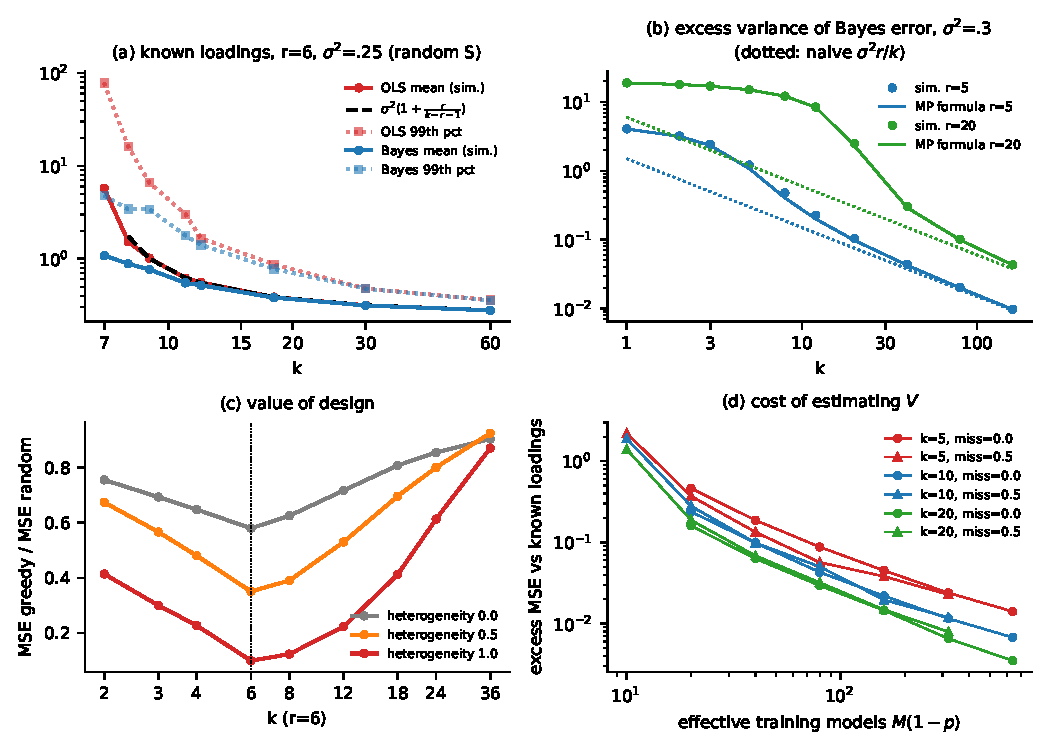
\includegraphics[width=.92\linewidth]{figs/fig_synthetic.pdf}
\caption{Synthetic checks of the theory (simulated data).}\label{fig:synth}
\end{figure}
\begin{figure}[h]
\centering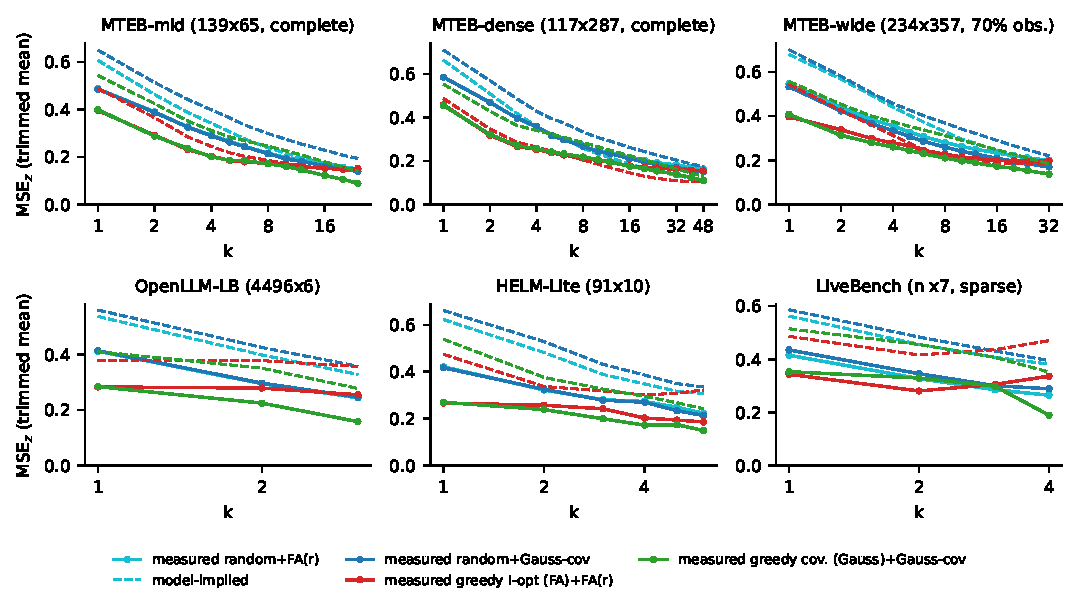
\includegraphics[width=\linewidth]{figs/fig_theory_vs_real.pdf}
\caption{Measured (solid) vs.\ model-implied (dashed) MSE$_z$ on real matrices, random split.}\label{fig:theoryreal}
\end{figure}
\begin{figure}[h]
\centering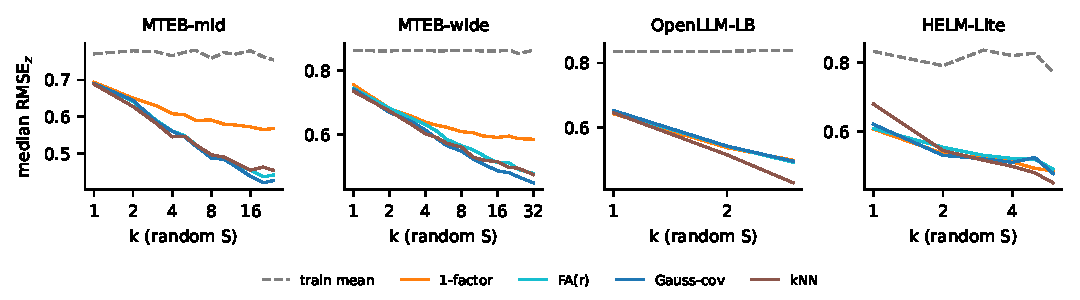
\includegraphics[width=\linewidth]{figs/fig_predictors.pdf}
\caption{Predictors with random subsets (family split, median $\rmse$).}\label{fig:pred}
\end{figure}
\begin{figure}[h]
\centering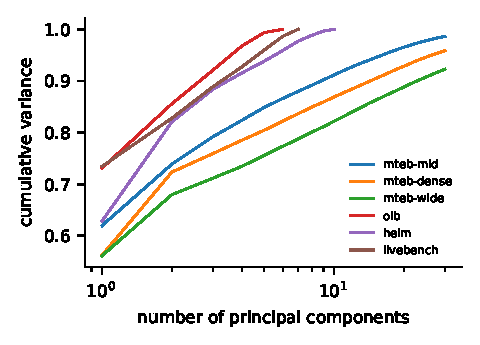
\includegraphics[width=.55\linewidth]{figs/fig_spectrum.pdf}
\caption{Cumulative variance of the correlation spectrum of each matrix.}\label{fig:spec}
\end{figure}
\begin{figure}[h]
\centering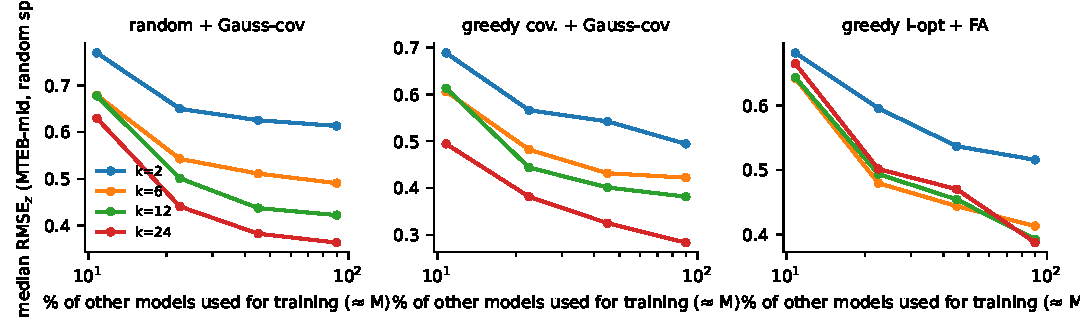
\includegraphics[width=\linewidth]{figs/fig_conditions.pdf}
\caption{MTEB-mid (random split): median $\rmse$ vs.\ fraction of training rows kept, for selected $k$.}\label{fig:cond}
\end{figure}
\begin{table}[h]
\caption{Generative-LLM leaderboards (family split), median $\rmse$ [95\% CI].}\label{tab:llm}
\centering\scriptsize\setlength{\tabcolsep}{3pt}\begin{tabular}{lrrr}\toprule
$k$ & 1 & 2 & 3 \\\midrule
\multicolumn{4}{l}{\textit{OpenLLM-LB (4496x6)}} \\
train mean & 0.836 \scriptsize[0.746,0.963] & 0.837 \scriptsize[0.744,0.965] & 0.840 \scriptsize[0.744,0.954] \\
random + Gauss & 0.653 \scriptsize[0.617,0.679] & 0.544 \scriptsize[0.515,0.570] & 0.497 \scriptsize[0.470,0.519] \\
random + FA & 0.649 \scriptsize[0.613,0.677] & 0.543 \scriptsize[0.514,0.567] & 0.494 \scriptsize[0.469,0.516] \\
greedy I-opt + FA & 0.524 \scriptsize[0.491,0.556] & 0.520 \scriptsize[0.485,0.551] & 0.492 \scriptsize[0.449,0.535] \\
greedy cov + Gauss & 0.528 \scriptsize[0.493,0.560] & 0.459 \scriptsize[0.425,0.492] & 0.385 \scriptsize[0.366,0.404] \\
\multicolumn{4}{l}{\textit{HELM-Lite (91x10)}} \\
train mean & 0.833 \scriptsize[0.667,0.889] & 0.791 \scriptsize[0.664,0.892] & 0.837 \scriptsize[0.653,0.912] \\
random + Gauss & 0.621 \scriptsize[0.560,0.742] & 0.531 \scriptsize[0.494,0.614] & 0.520 \scriptsize[0.448,0.636] \\
random + FA & 0.609 \scriptsize[0.565,0.743] & 0.554 \scriptsize[0.500,0.605] & 0.531 \scriptsize[0.439,0.623] \\
greedy I-opt + FA & 0.529 \scriptsize[0.465,0.580] & 0.477 \scriptsize[0.422,0.585] & 0.483 \scriptsize[0.410,0.506] \\
greedy cov + Gauss & 0.561 \scriptsize[0.473,0.627] & 0.528 \scriptsize[0.455,0.610] & 0.466 \scriptsize[0.384,0.578] \\
\multicolumn{4}{l}{\textit{LiveBench (n x7, sparse)}} \\
train mean & 0.881 \scriptsize[0.792,0.996] & 0.884 \scriptsize[0.787,0.996] & 0.860 \scriptsize[0.797,1.018] \\
random + Gauss & 0.679 \scriptsize[0.592,0.743] & 0.567 \scriptsize[0.536,0.634] & 0.555 \scriptsize[0.514,0.617] \\
random + FA & 0.672 \scriptsize[0.585,0.738] & 0.561 \scriptsize[0.516,0.639] & 0.538 \scriptsize[0.511,0.607] \\
greedy I-opt + FA & 0.572 \scriptsize[0.517,0.661] & 0.561 \scriptsize[0.509,0.617] & 0.536 \scriptsize[0.487,0.623] \\
greedy cov + Gauss & 0.571 \scriptsize[0.515,0.661] & 0.564 \scriptsize[0.516,0.671] & 0.511 \scriptsize[0.436,0.592] \\
\bottomrule\end{tabular}

\end{table}
\begin{table}[h]
\caption{Median mean-absolute error in benchmark score points (family split).}\label{tab:raw}
\centering\small\begin{tabular}{lrrrrr}\toprule
matrix & $k$ & train mean & random+Gauss & greedy cov+Gauss & greedy I-opt+FA \\\midrule
MTEB-mid & 4 & 9.43 & 5.84 & 4.61 & 4.47 \\
MTEB-mid & 8 & 9.58 & 4.95 & 4.42 & 4.15 \\
MTEB-mid & 24 & 9.36 & 4.04 & 3.61 & 4.08 \\
MTEB-dense & 4 & 8.39 & 5.45 & 4.37 & 4.24 \\
MTEB-dense & 8 & 8.39 & 4.53 & 4.01 & 3.90 \\
MTEB-dense & 24 & 8.34 & 3.76 & 3.52 & 3.57 \\
MTEB-wide & 4 & 10.79 & 6.41 & 5.24 & 5.63 \\
MTEB-wide & 8 & 10.81 & 5.56 & 4.82 & 4.98 \\
MTEB-wide & 24 & 10.79 & 4.59 & 4.30 & 4.51 \\
\bottomrule\end{tabular}

\end{table}
\begin{table}[h]
\caption{Stability across fold-assignment seeds and split type (MTEB-mid, median $\rmse$).}\label{tab:seeds}
\centering\small\begin{tabular}{lrrrrrr}\toprule
 & \multicolumn{2}{c}{random+Gauss} & \multicolumn{2}{c}{greedy cov+Gauss} & \multicolumn{2}{c}{greedy I-opt+FA} \\
 & $k$=4 & $k$=12 & $k$=4 & $k$=12 & $k$=4 & $k$=12 \\\midrule
family split, seed 0 & 0.560 & 0.467 & 0.470 & 0.405 & 0.486 & 0.431 \\
family split, seed 1 & 0.549 & 0.458 & 0.476 & 0.406 & 0.500 & 0.433 \\
family split, seed 2 & 0.558 & 0.448 & 0.485 & 0.399 & 0.457 & 0.435 \\
random split, seed 0 & 0.536 & 0.422 & 0.433 & 0.382 & 0.440 & 0.392 \\
\bottomrule\end{tabular}

\end{table}
\begin{table}[h]
\caption{Data-condition sweep, MTEB-mid, random split, median $\rmse$ (train-mean baseline $\approx0.74$ at full history; the baseline changes with the retained rows because standardisation is refit).}\label{tab:cond}
\centering\small\begin{tabular}{lrrrrrr}\toprule
 & \multicolumn{2}{c}{random+Gauss} & \multicolumn{2}{c}{greedy cov+Gauss} & \multicolumn{2}{c}{greedy I-opt+FA} \\
 & $k$=6 & $k$=12 & $k$=6 & $k$=12 & $k$=6 & $k$=12 \\\midrule
train rows kept: 12\% of rows ($M\approx$15) & 0.679 & 0.678 & 0.606 & 0.613 & 0.642 & 0.643 \\
train rows kept: 25\% ($M\approx$31) & 0.543 & 0.501 & 0.482 & 0.444 & 0.479 & 0.493 \\
train rows kept: 50\% ($M\approx$62) & 0.511 & 0.437 & 0.432 & 0.401 & 0.444 & 0.454 \\
train rows kept: 100\% ($M\approx$125) & 0.491 & 0.422 & 0.422 & 0.382 & 0.413 & 0.392 \\
\midrule
train cells masked: 30\% & 0.530 & 0.463 & 0.490 & 0.442 & 0.433 & 0.421 \\
train cells masked: 60\% & 0.617 & 0.581 & 0.576 & 0.551 & 0.490 & 0.503 \\
train cells masked: 80\% & 0.827 & 0.835 & 0.845 & 0.856 & 0.609 & 0.621 \\
\bottomrule\end{tabular}

\end{table}

\section{Benchmarks chosen by each rule (in-sample illustration)}\label{app:selected}
Fitted on all rows (not used in any accuracy claim). OLB: greedy I-opt MMLU-PRO, GPQA, MATH Lvl 5; greedy cov MMLU-PRO, IFEval, MUSR; communality BBH, MMLU-PRO, GPQA. HELM Lite ($k=4$): greedy cov MMLU, NarrativeQA, NaturalQuestions (closed-book), WMT 2014; communality MMLU, OpenbookQA, MedQA, NaturalQuestions (open-book). LiveBench: greedy cov coding\_completion, paraphrase, connections, typos. MTEB-mid ($k=6$, $r=8$): I-opt WikipediaRetrievalMultilingual, NFCorpus, MedrxivClusteringS2S.v2, STS15, AmazonReviewsClassification, MassiveScenarioClassification; communality MassiveScenarioClassification, BiorxivClusteringP2P.v2, MedrxivClusteringP2P.v2, MedrxivClusteringS2S.v2, STS14, CQADupstackGamingRetrieval. MTEB-dense: communality picks six CQADupstack subforum retrieval tasks. Full output: \texttt{results/summary\_selected.json}.

\section{Paired tests}\label{app:tests}
\texttt{results/summary\_paired\_tests.csv} lists, for each matrix, split, rule ($\in$\{greedy I-opt, greedy cov\}) and $k$, the number of held-out models, mean/median paired difference of $\rmse$ to random (Gauss-cov) and the Holm-adjusted Wilcoxon $p$-value over all comparisons. Because models of one family are dependent these $p$-values are optimistic; the cluster-bootstrap intervals in Table~\ref{tab:selgain} are the primary uncertainty statement.

\section{Compute, software, data licences}
CPU only (40 cores available; all experiments $\approx$ 40 min wall-clock; synthetic checks $\approx$ 3 min). Python 3.11, numpy 2.4, scipy 1.17, pandas 3.0, scikit-learn 1.9, pyarrow 26, joblib 1.6. MTEB results: CC0-1.0. Open LLM Leaderboard and LiveBench dataset cards declare no licence; HELM Lite data follow the licences of the underlying scenarios (not verified item-by-item); only aggregate score tables are used.

\newpage
\section*{NeurIPS Paper Checklist}




\begin{enumerate}

\item {\bf Claims}
    \item[] Question: Do the main claims made in the abstract and introduction accurately reflect the paper's contributions and scope?
    \item[] Answer: \answerYes{} % Replace by \answerYes{}, \answerNo{}, or \answerNA{}.
    \item[] Justification: Abstract and introduction state the hypotheses and findings, including which hold only partly (Sec.~5) and the scope limits (Sec.~6).
    \item[] Guidelines:
    \begin{itemize}
        \item The answer \answerNA{} means that the abstract and introduction do not include the claims made in the paper.
        \item The abstract and/or introduction should clearly state the claims made, including the contributions made in the paper and important assumptions and limitations. A \answerNo{} or \answerNA{} answer to this question will not be perceived well by the reviewers. 
        \item The claims made should match theoretical and experimental results, and reflect how much the results can be expected to generalize to other settings. 
        \item It is fine to include aspirational goals as motivation as long as it is clear that these goals are not attained by the paper. 
    \end{itemize}

\item {\bf Limitations}
    \item[] Question: Does the paper discuss the limitations of the work performed by the authors?
    \item[] Answer: \answerYes{} % Replace by \answerYes{}, \answerNo{}, or \answerNA{}.
    \item[] Justification: Section 6 lists ten limitations (embedding-benchmark data, tiny LLM leaderboards, selection effects, heavy tails, theory assumptions).
    \item[] Guidelines:
    \begin{itemize}
        \item The answer \answerNA{} means that the paper has no limitation while the answer \answerNo{} means that the paper has limitations, but those are not discussed in the paper. 
        \item The authors are encouraged to create a separate ``Limitations'' section in their paper.
        \item The paper should point out any strong assumptions and how robust the results are to violations of these assumptions (e.g., independence assumptions, noiseless settings, model well-specification, asymptotic approximations only holding locally). The authors should reflect on how these assumptions might be violated in practice and what the implications would be.
        \item The authors should reflect on the scope of the claims made, e.g., if the approach was only tested on a few datasets or with a few runs. In general, empirical results often depend on implicit assumptions, which should be articulated.
        \item The authors should reflect on the factors that influence the performance of the approach. For example, a facial recognition algorithm may perform poorly when image resolution is low or images are taken in low lighting. Or a speech-to-text system might not be used reliably to provide closed captions for online lectures because it fails to handle technical jargon.
        \item The authors should discuss the computational efficiency of the proposed algorithms and how they scale with dataset size.
        \item If applicable, the authors should discuss possible limitations of their approach to address problems of privacy and fairness.
        \item While the authors might fear that complete honesty about limitations might be used by reviewers as grounds for rejection, a worse outcome might be that reviewers discover limitations that aren't acknowledged in the paper. The authors should use their best judgment and recognize that individual actions in favor of transparency play an important role in developing norms that preserve the integrity of the community. Reviewers will be specifically instructed to not penalize honesty concerning limitations.
    \end{itemize}

\item {\bf Theory assumptions and proofs}
    \item[] Question: For each theoretical result, does the paper provide the full set of assumptions and a complete (and correct) proof?
    \item[] Answer: \answerYes{} % Replace by \answerYes{}, \answerNo{}, or \answerNA{}.
    \item[] Justification: Assumptions are stated before Propositions 1--2; proofs are in Appendix A; the Marchenko--Pastur part is explicitly asymptotic and checked by simulation.
    \item[] Guidelines:
    \begin{itemize}
        \item The answer \answerNA{} means that the paper does not include theoretical results. 
        \item All the theorems, formulas, and proofs in the paper should be numbered and cross-referenced.
        \item All assumptions should be clearly stated or referenced in the statement of any theorems.
        \item The proofs can either appear in the main paper or the supplemental material, but if they appear in the supplemental material, the authors are encouraged to provide a short proof sketch to provide intuition. 
        \item Inversely, any informal proof provided in the core of the paper should be complemented by formal proofs provided in appendix or supplemental material.
        \item Theorems and Lemmas that the proof relies upon should be properly referenced. 
    \end{itemize}

    \item {\bf Experimental result reproducibility}
    \item[] Question: Does the paper fully disclose all the information needed to reproduce the main experimental results of the paper to the extent that it affects the main claims and/or conclusions of the paper (regardless of whether the code and data are provided or not)?
    \item[] Answer: \answerYes{} % Replace by \answerYes{}, \answerNo{}, or \answerNA{}.
    \item[] Justification: Sec.~4 and the appendix give data versions, splits, hyper-parameter grids, seeds and the pipeline; the README lists every command.
    \item[] Guidelines:
    \begin{itemize}
        \item The answer \answerNA{} means that the paper does not include experiments.
        \item If the paper includes experiments, a \answerNo{} answer to this question will not be perceived well by the reviewers: Making the paper reproducible is important, regardless of whether the code and data are provided or not.
        \item If the contribution is a dataset and\slash or model, the authors should describe the steps taken to make their results reproducible or verifiable. 
        \item Depending on the contribution, reproducibility can be accomplished in various ways. For example, if the contribution is a novel architecture, describing the architecture fully might suffice, or if the contribution is a specific model and empirical evaluation, it may be necessary to either make it possible for others to replicate the model with the same dataset, or provide access to the model. In general. releasing code and data is often one good way to accomplish this, but reproducibility can also be provided via detailed instructions for how to replicate the results, access to a hosted model (e.g., in the case of a large language model), releasing of a model checkpoint, or other means that are appropriate to the research performed.
        \item While NeurIPS does not require releasing code, the conference does require all submissions to provide some reasonable avenue for reproducibility, which may depend on the nature of the contribution. For example
        \begin{enumerate}
            \item If the contribution is primarily a new algorithm, the paper should make it clear how to reproduce that algorithm.
            \item If the contribution is primarily a new model architecture, the paper should describe the architecture clearly and fully.
            \item If the contribution is a new model (e.g., a large language model), then there should either be a way to access this model for reproducing the results or a way to reproduce the model (e.g., with an open-source dataset or instructions for how to construct the dataset).
            \item We recognize that reproducibility may be tricky in some cases, in which case authors are welcome to describe the particular way they provide for reproducibility. In the case of closed-source models, it may be that access to the model is limited in some way (e.g., to registered users), but it should be possible for other researchers to have some path to reproducing or verifying the results.
        \end{enumerate}
    \end{itemize}


\item {\bf Open access to data and code}
    \item[] Question: Does the paper provide open access to the data and code, with sufficient instructions to faithfully reproduce the main experimental results, as described in supplemental material?
    \item[] Answer: \answerYes{} % Replace by \answerYes{}, \answerNo{}, or \answerNA{}.
    \item[] Justification: Code, pinned data-fetch steps and processed matrices are in the supplementary repository (README.md); data are public.
    \item[] Guidelines:
    \begin{itemize}
        \item The answer \answerNA{} means that paper does not include experiments requiring code.
        \item Please see the NeurIPS code and data submission guidelines (\url{https://neurips.cc/public/guides/CodeSubmissionPolicy}) for more details.
        \item While we encourage the release of code and data, we understand that this might not be possible, so \answerNo{} is an acceptable answer. Papers cannot be rejected simply for not including code, unless this is central to the contribution (e.g., for a new open-source benchmark).
        \item The instructions should contain the exact command and environment needed to run to reproduce the results. See the NeurIPS code and data submission guidelines (\url{https://neurips.cc/public/guides/CodeSubmissionPolicy}) for more details.
        \item The authors should provide instructions on data access and preparation, including how to access the raw data, preprocessed data, intermediate data, and generated data, etc.
        \item The authors should provide scripts to reproduce all experimental results for the new proposed method and baselines. If only a subset of experiments are reproducible, they should state which ones are omitted from the script and why.
        \item At submission time, to preserve anonymity, the authors should release anonymized versions (if applicable).
        \item Providing as much information as possible in supplemental material (appended to the paper) is recommended, but including URLs to data and code is permitted.
    \end{itemize}


\item {\bf Experimental setting/details}
    \item[] Question: Does the paper specify all the training and test details (e.g., data splits, hyperparameters, how they were chosen, type of optimizer) necessary to understand the results?
    \item[] Answer: \answerYes{} % Replace by \answerYes{}, \answerNo{}, or \answerNA{}.
    \item[] Justification: Sec.~3--4 and Appendix E give splits, grids, tuning procedure and settings; tuning uses training rows only.
    \item[] Guidelines:
    \begin{itemize}
        \item The answer \answerNA{} means that the paper does not include experiments.
        \item The experimental setting should be presented in the core of the paper to a level of detail that is necessary to appreciate the results and make sense of them.
        \item The full details can be provided either with the code, in appendix, or as supplemental material.
    \end{itemize}

\item {\bf Experiment statistical significance}
    \item[] Question: Does the paper report error bars suitably and correctly defined or other appropriate information about the statistical significance of the experiments?
    \item[] Answer: \answerYes{} % Replace by \answerYes{}, \answerNo{}, or \answerNA{}.
    \item[] Justification: Family-cluster bootstrap 95\% intervals (1000 resamples), fold-seed variation (appendix seeds table), and Holm-corrected paired tests are reported; limits of independence are stated.
    \item[] Guidelines:
    \begin{itemize}
        \item The answer \answerNA{} means that the paper does not include experiments.
        \item The authors should answer \answerYes{} if the results are accompanied by error bars, confidence intervals, or statistical significance tests, at least for the experiments that support the main claims of the paper.
        \item The factors of variability that the error bars are capturing should be clearly stated (for example, train/test split, initialization, random drawing of some parameter, or overall run with given experimental conditions).
        \item The method for calculating the error bars should be explained (closed form formula, call to a library function, bootstrap, etc.)
        \item The assumptions made should be given (e.g., Normally distributed errors).
        \item It should be clear whether the error bar is the standard deviation or the standard error of the mean.
        \item It is OK to report 1-sigma error bars, but one should state it. The authors should preferably report a 2-sigma error bar than state that they have a 96\% CI, if the hypothesis of Normality of errors is not verified.
        \item For asymmetric distributions, the authors should be careful not to show in tables or figures symmetric error bars that would yield results that are out of range (e.g., negative error rates).
        \item If error bars are reported in tables or plots, the authors should explain in the text how they were calculated and reference the corresponding figures or tables in the text.
    \end{itemize}

\item {\bf Experiments compute resources}
    \item[] Question: For each experiment, does the paper provide sufficient information on the computer resources (type of compute workers, memory, time of execution) needed to reproduce the experiments?
    \item[] Answer: \answerYes{} % Replace by \answerYes{}, \answerNo{}, or \answerNA{}.
    \item[] Justification: Appendix E: CPU only, about 40 minutes wall-clock on 40 cores for all real-data experiments.
    \item[] Guidelines:
    \begin{itemize}
        \item The answer \answerNA{} means that the paper does not include experiments.
        \item The paper should indicate the type of compute workers CPU or GPU, internal cluster, or cloud provider, including relevant memory and storage.
        \item The paper should provide the amount of compute required for each of the individual experimental runs as well as estimate the total compute. 
        \item The paper should disclose whether the full research project required more compute than the experiments reported in the paper (e.g., preliminary or failed experiments that didn't make it into the paper). 
    \end{itemize}
    
\item {\bf Code of ethics}
    \item[] Question: Does the research conducted in the paper conform, in every respect, with the NeurIPS Code of Ethics \url{https://neurips.cc/public/EthicsGuidelines}?
    \item[] Answer: \answerYes{} % Replace by \answerYes{}, \answerNo{}, or \answerNA{}.
    \item[] Justification: Only public leaderboard score tables and simulated data are used; no human subjects or sensitive data.
    \item[] Guidelines:
    \begin{itemize}
        \item The answer \answerNA{} means that the authors have not reviewed the NeurIPS Code of Ethics.
        \item If the authors answer \answerNo, they should explain the special circumstances that require a deviation from the Code of Ethics.
        \item The authors should make sure to preserve anonymity (e.g., if there is a special consideration due to laws or regulations in their jurisdiction).
    \end{itemize}


\item {\bf Broader impacts}
    \item[] Question: Does the paper discuss both potential positive societal impacts and negative societal impacts of the work performed?
    \item[] Answer: \answerNA{} % Replace by \answerYes{}, \answerNo{}, or \answerNA{}.
    \item[] Justification: The work analyses public benchmark scores; no direct societal-impact pathway beyond general evaluation practice is identified.
    \item[] Guidelines:
    \begin{itemize}
        \item The answer \answerNA{} means that there is no societal impact of the work performed.
        \item If the authors answer \answerNA{} or \answerNo, they should explain why their work has no societal impact or why the paper does not address societal impact.
        \item Examples of negative societal impacts include potential malicious or unintended uses (e.g., disinformation, generating fake profiles, surveillance), fairness considerations (e.g., deployment of technologies that could make decisions that unfairly impact specific groups), privacy considerations, and security considerations.
        \item The conference expects that many papers will be foundational research and not tied to particular applications, let alone deployments. However, if there is a direct path to any negative applications, the authors should point it out. For example, it is legitimate to point out that an improvement in the quality of generative models could be used to generate Deepfakes for disinformation. On the other hand, it is not needed to point out that a generic algorithm for optimizing neural networks could enable people to train models that generate Deepfakes faster.
        \item The authors should consider possible harms that could arise when the technology is being used as intended and functioning correctly, harms that could arise when the technology is being used as intended but gives incorrect results, and harms following from (intentional or unintentional) misuse of the technology.
        \item If there are negative societal impacts, the authors could also discuss possible mitigation strategies (e.g., gated release of models, providing defenses in addition to attacks, mechanisms for monitoring misuse, mechanisms to monitor how a system learns from feedback over time, improving the efficiency and accessibility of ML).
    \end{itemize}
    
\item {\bf Safeguards}
    \item[] Question: Does the paper describe safeguards that have been put in place for responsible release of data or models that have a high risk for misuse (e.g., pre-trained language models, image generators, or scraped datasets)?
    \item[] Answer: \answerNA{} % Replace by \answerYes{}, \answerNo{}, or \answerNA{}.
    \item[] Justification: No model or data with misuse risk is released.
    \item[] Guidelines:
    \begin{itemize}
        \item The answer \answerNA{} means that the paper poses no such risks.
        \item Released models that have a high risk for misuse or dual-use should be released with necessary safeguards to allow for controlled use of the model, for example by requiring that users adhere to usage guidelines or restrictions to access the model or implementing safety filters. 
        \item Datasets that have been scraped from the Internet could pose safety risks. The authors should describe how they avoided releasing unsafe images.
        \item We recognize that providing effective safeguards is challenging, and many papers do not require this, but we encourage authors to take this into account and make a best faith effort.
    \end{itemize}

\item {\bf Licenses for existing assets}
    \item[] Question: Are the creators or original owners of assets (e.g., code, data, models), used in the paper, properly credited and are the license and terms of use explicitly mentioned and properly respected?
    \item[] Answer: \answerYes{} % Replace by \answerYes{}, \answerNo{}, or \answerNA{}.
    \item[] Justification: Sources, commits and licences are listed in Sec.~4 and Appendix E; licences for the Open LLM Leaderboard, LiveBench and HELM scenario data are undeclared or unverified and this is stated.
    \item[] Guidelines:
    \begin{itemize}
        \item The answer \answerNA{} means that the paper does not use existing assets.
        \item The authors should cite the original paper that produced the code package or dataset.
        \item The authors should state which version of the asset is used and, if possible, include a URL.
        \item The name of the license (e.g., CC-BY 4.0) should be included for each asset.
        \item For scraped data from a particular source (e.g., website), the copyright and terms of service of that source should be provided.
        \item If assets are released, the license, copyright information, and terms of use in the package should be provided. For popular datasets, \url{paperswithcode.com/datasets} has curated licenses for some datasets. Their licensing guide can help determine the license of a dataset.
        \item For existing datasets that are re-packaged, both the original license and the license of the derived asset (if it has changed) should be provided.
        \item If this information is not available online, the authors are encouraged to reach out to the asset's creators.
    \end{itemize}

\item {\bf New assets}
    \item[] Question: Are new assets introduced in the paper well documented and is the documentation provided alongside the assets?
    \item[] Answer: \answerYes{} % Replace by \answerYes{}, \answerNo{}, or \answerNA{}.
    \item[] Justification: Code and processed score matrices (derived from public data) are documented in the README.
    \item[] Guidelines:
    \begin{itemize}
        \item The answer \answerNA{} means that the paper does not release new assets.
        \item Researchers should communicate the details of the dataset\slash code\slash model as part of their submissions via structured templates. This includes details about training, license, limitations, etc. 
        \item The paper should discuss whether and how consent was obtained from people whose asset is used.
        \item At submission time, remember to anonymize your assets (if applicable). You can either create an anonymized URL or include an anonymized zip file.
    \end{itemize}

\item {\bf Crowdsourcing and research with human subjects}
    \item[] Question: For crowdsourcing experiments and research with human subjects, does the paper include the full text of instructions given to participants and screenshots, if applicable, as well as details about compensation (if any)? 
    \item[] Answer: \answerNA{} % Replace by \answerYes{}, \answerNo{}, or \answerNA{}.
    \item[] Justification: No crowdsourcing or human-subject research.
    \item[] Guidelines:
    \begin{itemize}
        \item The answer \answerNA{} means that the paper does not involve crowdsourcing nor research with human subjects.
        \item Including this information in the supplemental material is fine, but if the main contribution of the paper involves human subjects, then as much detail as possible should be included in the main paper. 
        \item According to the NeurIPS Code of Ethics, workers involved in data collection, curation, or other labor should be paid at least the minimum wage in the country of the data collector. 
    \end{itemize}

\item {\bf Institutional review board (IRB) approvals or equivalent for research with human subjects}
    \item[] Question: Does the paper describe potential risks incurred by study participants, whether such risks were disclosed to the subjects, and whether Institutional Review Board (IRB) approvals (or an equivalent approval/review based on the requirements of your country or institution) were obtained?
    \item[] Answer: \answerNA{} % Replace by \answerYes{}, \answerNo{}, or \answerNA{}.
    \item[] Justification: No human-subject research.
    \item[] Guidelines:
    \begin{itemize}
        \item The answer \answerNA{} means that the paper does not involve crowdsourcing nor research with human subjects.
        \item Depending on the country in which research is conducted, IRB approval (or equivalent) may be required for any human subjects research. If you obtained IRB approval, you should clearly state this in the paper. 
        \item We recognize that the procedures for this may vary significantly between institutions and locations, and we expect authors to adhere to the NeurIPS Code of Ethics and the guidelines for their institution. 
        \item For initial submissions, do not include any information that would break anonymity (if applicable), such as the institution conducting the review.
    \end{itemize}

\item {\bf Declaration of LLM usage}
    \item[] Question: Does the paper describe the usage of LLMs if it is an important, original, or non-standard component of the core methods in this research? Note that if the LLM is used only for writing, editing, or formatting purposes and does \emph{not} impact the core methodology, scientific rigor, or originality of the research, declaration is not required.
    %this research? 
    \item[] Answer: \answerNA{} % Replace by \answerYes{}, \answerNo{}, or \answerNA{}.
    \item[] Justification: LLMs were not a component of the research method; an AI research assistant was used for coding and drafting and all reported numbers come from the released code.
    \item[] Guidelines:
    \begin{itemize}
        \item The answer \answerNA{} means that the core method development in this research does not involve LLMs as any important, original, or non-standard components.
        \item Please refer to our LLM policy in the NeurIPS handbook for what should or should not be described.
    \end{itemize}

\end{enumerate}
\end{document}
